\section{Материалы предварительного проектирования системы}
\subsection{Функциональная схема обработки данных}

\begin{figure}[!htb]
    \centering
    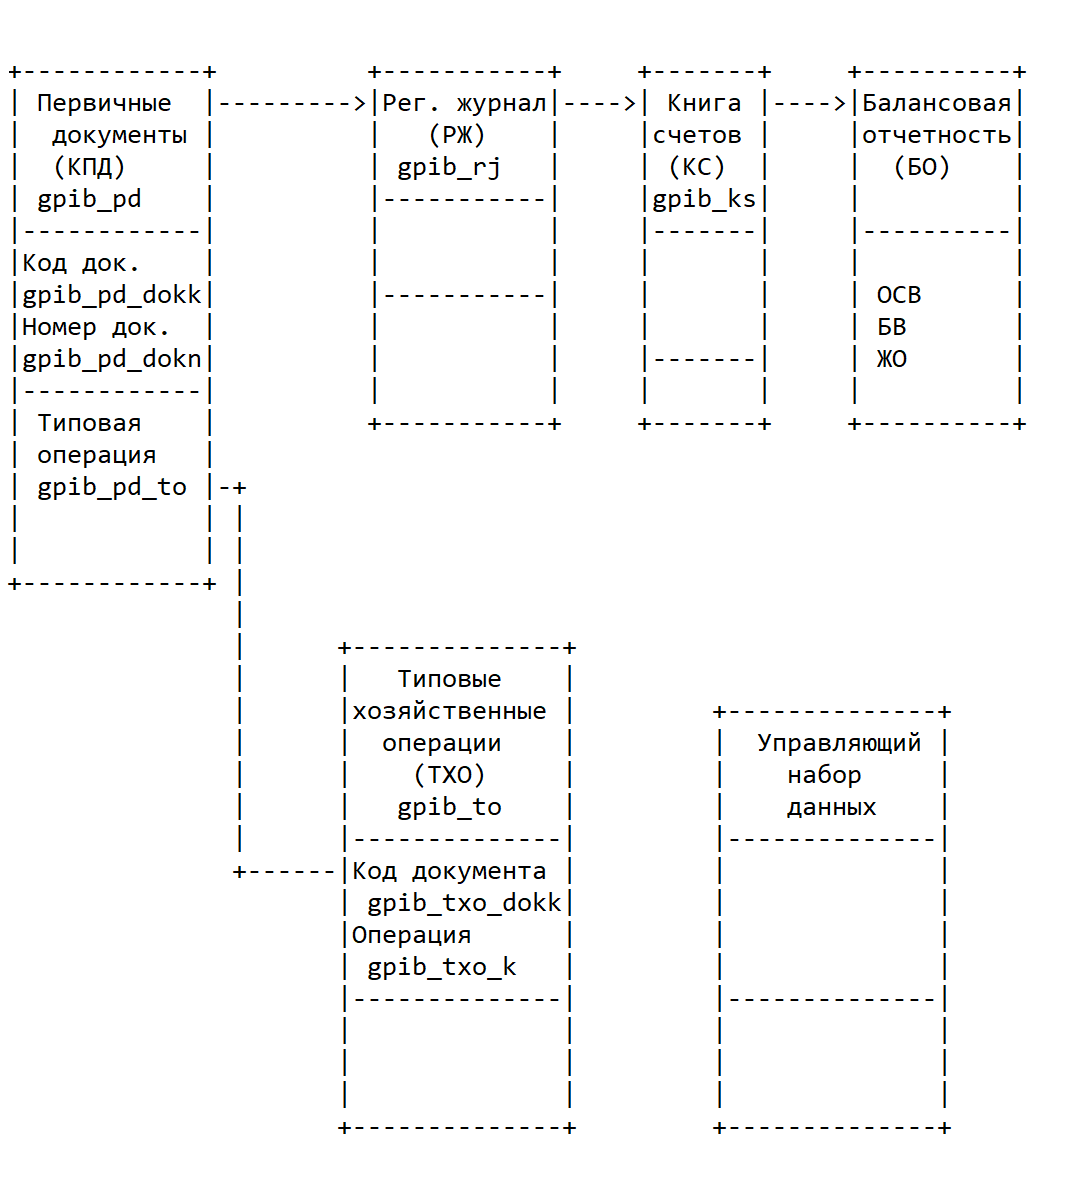
\includegraphics[height=11cm]
        {_assets/gpib_part2.png}
    \caption{Функциональная схема обработки данных}
    \label{fig:gpib_part2}
\end{figure}

\subsection{Описание картотек}

Картотеки:

\begin{itemize}
    \item Первичные документы gpib\_pd;
    \item Регистрационный журнал (РЖ) gpib\_rj;
    \item Книга счетов(КС) gpib\_ks;
    \item Типовые хозяйственные операции (ТХО) gpib\_to.
\end{itemize}

\begin{table}[!htbp]
    \centering
    \scriptsize
    \caption{Первичные документы gpib\_pd}
    \begin{tabular}{|l|l|l|} 

                                                                                   \hline
\textbf{Реквизит}           &\textbf{Обозначение}   &\textbf{Тип и значность}   \\ \hline
поле связи =0               &gpib\_pd\_0            &n1                         \\ \hline
код документа < --- opd     &gpib\_pd\_dokk         &c3                         \\ \hline
номер документа             &gpib\_pd\_dokn         &n5                         \\ \hline
дата документа              &gpib\_pd\_dokd         &d8                         \\ \hline
типовая операция < --- txo  &gpib\_pd\_to           &c10                        \\ \hline
дебет *txo                  &gpib\_pd\_db           &n2                         \\ \hline
дебет наименование *txo     &gpib\_pd\_dbn          &c10                        \\ \hline
кредит *txo                 &gpib\_pd\_kr           &n2                         \\ \hline
кредит наименование *txo    &gpib\_pd\_krn          &c10                        \\ \hline
сумма                       &gpib\_pd\_rub          &n10                        \\ \hline

    \end{tabular}
\end{table}

% \begin{table}[h!p]
%     \centering
%     \scriptsize
%     \caption{Виды аналитики gpia\_va}
%     \begin{tabular}{|l|l|l|} 

%                                                                                \hline
% \textbf{Реквизит}       &\textbf{Обозначение}   &\textbf{Тип и значность}   \\ \hline
% поле связи  	  =0    &gpia\_va\_0            &c1                         \\ \hline
% вид аналитики           &gpia\_va\_k            &c3                         \\ \hline
% название вида аналитики &gpia\_va\_n            &c15                        \\ \hline

%     \end{tabular}
% \end{table}

\begin{table}[!htbp]
    \centering
    \scriptsize
    \caption{Регистрационный журнал (РЖ) gpib\_rj}
    \begin{tabular}{|l|l|l|} 

                                                                                       \hline
\textbf{Реквизит}               &\textbf{Обозначение}   &\textbf{Тип и значность}   \\ \hline
поле связи =0                   &gpib\_rj\_0            &n1                         \\ \hline
дата операции                   &gpib\_rj\_data         &d8                         \\ \hline
код оправдательного документа   &gpib\_rj\_dokk         &c3                         \\ \hline
номер документа                 &gpib\_rj\_dokn         &n10                        \\ \hline
дата документа                  &gpib\_rj\_dokd         &d8                         \\ \hline
содержание операции             &gpib\_rj\_to           &c10                        \\ \hline
дебет, счет                     &gpib\_rj\_db           &n2                         \\ \hline
дебет, наименование             &gpib\_rj\_dbn          &c10                        \\ \hline
кредит, счет                    &gpib\_rj\_kr           &n2                         \\ \hline
кредит наименование             &gpib\_rj\_krn          &c10                        \\ \hline
сумма                           &gpib\_rj\_rub          &n10                        \\ \hline

    \end{tabular}
\end{table}

\begin{table}[!htbp]
    \centering
    \scriptsize
    \caption{Книга счетов(КС) gpib\_ks}
    \begin{tabular}{|l|l|l|} 

                                                                                       \hline
\textbf{Реквизит}               &\textbf{Обозначение}   &\textbf{Тип и значность}   \\ \hline
поле связи =0                   &gpib\_ks\_0            &n1                         \\ \hline
дата операции                   &gpib\_ks\_data         &d8                         \\ \hline
код оправдательного документа   &gpib\_ks\_dokk         &c3                         \\ \hline
номер документа                 &gpib\_ks\_dokn         &n10                        \\ \hline
дата документа                  &gpib\_ks\_dokd         &d8                         \\ \hline
операции                        &gpib\_ks\_to           &c10                        \\ \hline
счет                            &gpib\_ks\_s            &n2                         \\ \hline
счёт наименование               &gpib\_ks\_sn           &c10                        \\ \hline
кор. счёт                       &gpib\_ks\_ks           &n2                         \\ \hline
кор. счет наименование          &gpib\_ks\_ksn          &c10                        \\ \hline
сумма дб                        &gpib\_ks\_rubdb        &n10                        \\ \hline
сумма кр                        &gpib\_ks\_rubkr        &n10                        \\ \hline

    \end{tabular}
\end{table}

% \begin{table}[h!p]
%     \centering
%     \scriptsize
%     \caption{Определение первичных документов gpia\_opd}
%     \begin{tabular}{|l|l|l|} 

%                                                                                    \hline
% \textbf{Реквизит}           &\textbf{Обозначение}   &\textbf{Тип и значность}   \\ \hline
% поле связи       =0         &gpia\_opd\_0           &c1                         \\ \hline
% код документа               &gpia\_opd\_k           &c3                         \\ \hline
% наименование документа      &gpia\_opd\_n           &c10                        \\ \hline
% вид аналитики 1  < ---  va  &gpia\_opd\_av1         &c3                         \\ \hline
% тип аналитики 1    =д, к, x &gpia\_opd\_avt1        &c1                         \\ \hline
% виды аналитики 2            &gpia\_opd\_av2         &c3                         \\ \hline
% тип аналитики 2             &gpia\_opd\_avt2        &c1                         \\ \hline
% вид аналитики 3             &gpia\_opd\_av3         &c3                         \\ \hline
% тип аналитики 2             &gpia\_opd\_avt3        &c1                         \\ \hline

%     \end{tabular}
% \end{table}

\begin{table}[!htbp]
    \centering
    \scriptsize
    \caption{Типовые хозяйственные операции(ТХО) gpib\_txo}
    \begin{tabular}{|l|l|l|} 

                                                                                       \hline
\textbf{Реквизит}               &\textbf{Обозначение}   &\textbf{Тип и значность}   \\ \hline
поле связи =0                   &gpi\_to\_0             &n1                         \\ \hline
код документа < --- opd         &gpi\_to\_dokk          &c3                         \\ \hline
код типовой операции            &gpi\_to\_k             &c10                        \\ \hline
дебет, счёт < --- ps\_1         &gpi\_to\_db            &n2                         \\ \hline
дебет, наименование * ps\_1     &gpi\_to\_dbn           &c10                        \\ \hline
кредит < --- ps\_2              &gpi\_to\_kr            &n2                         \\ \hline
кредит, наименование * ps\_2    &gpi\_to\_krn           &c10                        \\ \hline

    \end{tabular}
\end{table}

% \begin{table}[h!p]
%     \centering
%     \scriptsize
%     \caption{План счетов(ПС) gpia\_ps}
%     \begin{tabular}{|l|l|l|} 

%                                                                                            \hline
% \textbf{Реквизит}                   &\textbf{Обозначение}   &\textbf{Тип и значность}   \\ \hline
% поле связи        =0                &gpia\_ps\_0            &c1                         \\ \hline
% счет                                &gpia\_ps\_s            &n2                         \\ \hline
% название счета                      &gpia\_ps\_n            &c10                        \\ \hline
% тип счета          = а, п, x        &gpia\_ps\_typ          &c1                         \\ \hline
% вид аналитики 1 из VA               &gpia\_ps\_av1          &c3                         \\ \hline
% вид аналитики 2 из VA               &gpia\_ps\_av2          &c3                         \\ \hline

%     \end{tabular}
% \end{table}

% \begin{table}[h!p]
%     \centering
%     \scriptsize
%     \caption{Коды аналитического учёта(КАУ) gpia\_kau}
%     \begin{tabular}{|l|l|l|} 

%                                                                                \hline
% \textbf{Реквизит}       &\textbf{Обозначение}   &\textbf{Тип и значность}   \\ \hline
% поле связи          =0  &gpia\_kau\_0           &c1                         \\ \hline
% вид аналитики           &gpia\_kau\_k           &c5                         \\ \hline
% вид аналитики           &gpia\_kau\_n           &c15                        \\ \hline

%     \end{tabular}
% \end{table}

% \begin{table}[h!p]
%     \centering
%     \scriptsize
%     \caption{Настройки системы gpia\_nst}
%     \begin{tabular}{|l|l|l|} 

%                                                                                \hline
% \textbf{Реквизит}       &\textbf{Обозначение}   &\textbf{Тип и значность}   \\ \hline
% поле связи          =0  &gpia\_nst\_0           &c1                         \\ \hline
% дата текущая            &gpia\_nst\_datat       &D                          \\ \hline
% интервал с              &gpia\_nst\_datas       &D                          \\ \hline
% интервал до             &gpia\_nst\_datado      &D                          \\ \hline
% cчёт                    &gpia\_nst\_s           &n2                         \\ \hline
% название счёта          &gpia\_nst\_sn          &c10                        \\ \hline
% название фирмы          &gpia\_nst\_firma       &c10                        \\ \hline

%     \end{tabular}
% \end{table}

\newpage

\subsection{Описание работ}

\begin{table}[!htb]
    \centering
    \scriptsize
    \caption{Описание работ}
    \begin{tabular}{|p{8cm}|p{8cm}|} 

% = = = = = = = = = =

\hline

% = = = = = = = = = =

\textbf{Группа работ}
&
\textbf{Работы}
\\ \hline

% = = = = = = = = = =

Формирование и разноска первичных документов \par
\hspace{0pt} \par
\textbf{gpib\_Документы}
&
- gpib\_Ввод текущей даты \par
- gpib\_Ввод и разноска первичных документов(ПД)
\\ \hline

% = = = = = = = = = =

Работа с регистрационным журналом \par
\hspace{0pt} \par
\textbf{gpib\_РЖ}
&
- gpib\_Просмотр РЖ \par
- gpib\_Формирование КС и РЖ \par
- gpib\_Просмотр КС \par
- gpib\_Сформировать КС на печать \par
- gpib\_Просмотр КС для печати
\\ \hline

% = = = = = = = = = =

Формирование балансовой отчетности \par
\hspace{0pt} \par
\textbf{gpib\_БО}
&
- gpib\_Опеделение отчетных форм \par
- gpib\_сформировать КС на печать \par
- gpib\_ Просмотр КС для печати \par
- gpib\_Сформировать ОСВ \par
- gpib\_Просмотр ОСВ \par
- gpib\_Сформировать Ж-О \par
- gpib\_ Просмотр Ж-О \par
- gpib\_Сформировать БВ \par
- gpib\_ Просмотр БВ
\\ \hline

% = = = = = = = = = =

Сопровождение картотек-справочников \par
\hspace{0pt} \par
\textbf{gpib\_Картотеки}
&
- gpib\_Определение первичных документов \par
- gpib\_Типовые хозяйственные операции(ТХО) \par
- gpib\_Настройка АРМа
\\ \hline

% = = = = = = = = = =

Ведение архивов \par
\hspace{0pt} \par
\textbf{gpib\_Архивы}
&
- gpib\_Копия АРМ \par
- gpib\_Восстановление АРМ
\\ \hline

% = = = = = = = = = =

Выход из системы \par
\hspace{0pt} \par
\textbf{gpib\_Выход}
&
- gpib\_Выход из системы
\\ \hline

% = = = = = = = = = =

    \end{tabular}
\end{table}

\newpage
